\chapter{ORGANIZAÇÃO DIDÁTICO PEDAGÓGICA}

Curso Superior de Engenharia Eletrônica do Câmpus Toledo da UTFPR  é estruturado de acordo com: a Lei nº 9.131, de 24 de novembro de 1995 \cite{Lei:9131:1995}; a Lei nº 9.394, de 20 de dezembro de 1996 \cite{Lei:9394:1996}; a Lei nº 11.184, de 7 de outubro de 2005 \cite{Lei:11.184:2005}; o Estatuto e Regimento Geral da UTFPR \cite{estatutoutfpr}; as Diretrizes Curriculares Nacionais do Curso de Graduação em Engenharia \cite{dcneng}; a Resolução nº 90/2018 – COGEP \cite{cogep90}; e às demais diretrizes e regulamentos internos aplicáveis. A concepção de ensino e aprendizagem do curso, a matriz curricular, os procedimentos de avaliação e os instrumentos de apoio expressos no Projeto Pedagógico de Curso (PPC), são construídos coletivamente e submetidos ao Conselho de Graduação e Educação Profissional (COGEP) para aprovação, em modelo e prazo estabelecido.

Segundo o PPI:

\begin{citacao}
	``A  UTFPR  deve  contribuir  para  o  avanço  conceitual  da educação profissional e tecnológica, tomando como princípio a formação integral do homem,  em  bases  científicas  e  ético-políticas,  entendendo  que  o  exercício  das atividades humanas não se restringe ao caráter produtivo, mas compreende todas as dimensões: social, política, cultural e ambiental'' \cite{ppiutfpr}.
\end{citacao}

\pdfmarkupcomment{Complementar...}{Complementar de acordo com o texto norteador}

\pdfmarkupcomment{O Curso de Engenharia Eletrônica promove a aprendizagem de conhecimentos estruturados vinculados ao desenvolvimento de competências, em uma dinâmica que enfatiza a prática profissional sem excluir as dimensões sociais e ambientais da qual faz parte. As disciplinas, não mais isoladas, são promotoras do saber, saber fazer e saber ser, se responsabilizando pelo currículo vivo formador de profissionais aptos a mobilizar, integrar e aplicar adequadamente esses conhecimentos. A metodologia do curso envolve processos de participação do estudante que permite a constante construção do conhecimento.}{Retirado do PPC de Tecnologia de alimentos.}

Os conceitos são apresentados a partir dos conhecimentos expostos em livros didáticos, artigos científicos, situações reais e outros materiais bibliográficos pertinentes, conduzidos pela experiência dos(as) professor(as). Também são incentivados projetos que permitam a análise reflexiva e o aprendizado da prática profissional pelo discente. Procura-se continuamente estabelecer a interdisciplinaridade relacionando os conteúdos das diversas disciplinas que compõem o curso.

Dessa forma, a estrutura curricular do Curso de Engenharia Eletrônica da UTFPR – Campus Toledo tem base na demanda do mercado regional, demanda essa tanto de qualificação profissional, como de características socioeconômicas. Para dar atendimento à demanda do mercado de um profissional com um perfil diferenciado, não só em tecnologia, mas também voltado para o desenvolvimento social e sustentabilidade, a organização do Curso de Engenharia Eletrônica apresenta bases científicas e de gestão de nível superior dimensionada e direcionada às terminalidades da formação do engenheiro.

A matriz curricular do curso de Engenharia Eletrônica da UTFPR é estruturada em dez semestres sob o regime de matrícula por disciplina com entrada anual de 88 acadêmicos. Sua carga horária totaliza \pdfmarkupcomment{4060 h}{atualizar ao final} de atividades com conteúdo de natureza profissionalizante, científica, humanística, extensionista e cultural.

A organização da matriz curricular do curso contempla os objetivos de instigar o interesse pela ciência e tecnologia e, ao mesmo tempo, fornece um sólido embasamento para o conteúdo profissionalizante. Isto é alcançado apresentando disciplinas profissionalizantes o mais cedo possível, ao mesmo tempo que o aluno tem uma prévia do que será ministrado adiante no curso através da disciplina de Introdução à Engenharia. A maioria das disciplinas possui carga horária em laboratório, com experimentos realizados nas áreas de física, química e eletrônica desde o primeiro semestre. As disciplinas da área de formação profissionalizante estão presentes em todos os semestres e são desenvolvidas em sua maior parte em laboratório. Especificamente, os conteúdos de computação são apresentados desde o primeiro semestre, enquanto os conteúdos de engenharia elétrica e eletrônica são apresentados desde o terceiro. Além disso, a sequência de pré-requisitos das disciplinas permite a inclusão de atividades interdisciplinares desde o início do curso.

As atividades acadêmicas são divididas em AT (Atividades Teóricas) e AP (Atividades Práticas). As AT consistem na apresentação de conteúdos teóricos em sala de aula. Já as AP têm vistas ao desenvolvimento prático dos conteúdos, consistindo de experimentos, atividades de laboratório, ou visitas técnicas.

\nomenclature[A]{AT}{Atividades Teóricas}
\nomenclature[A]{AP}{Atividades Práticas} 

\pdfmarkupcomment{Os projetos pedagógicos dos cursos da UTFPR devem dar ênfase a AP. Para cursos de engenharia, a carga horária de AP, para o conjunto de disciplinas específicas, deve ser de, no mínimo, a metade. Objetiva-se, com isto, formar um profissional diferenciado, apto a lidar com problemas de ordem prática e pronto para lidar com as necessidades imediatas do mercado de trabalho.}{Acho que as diretrizes atuais não delimitam a quantidade de horas práticas}

\section{ORGANIZAÇÃO CURRICULAR}

%A Construção curricular deve responder diretamente aos objetivos formativos. Considerando as metas educacionais para formação profissional percebe-se que para alcança-las os projetos de ensino superior precisam propor mudanças significativas e inovadoras em suas organizações curriculares.

%Assim, é imperativo a construção de currículos inovadores e estrategicamente orientados à aprendizagem significativa, ao desenvolvimento integrado e sustentável, às necessidades, aspirações e expectativas dos alunos e à transformação da realidade em que vivem.

%No início da apresentação da organização curricular deve conter a proposta que fundamenta o curso, pois, são os fundamentos teórico metodológicos que sustentam as decisões sobre a escolha entre uma ou outra matriz curricular. A organização curricular do curso deve apresentar as unidades curriculares agrupadas por áreas de conhecimento, número de períodos, organização de temas transversais, integração horizontal e vertical. Incluir aqui como será desenvolvido no curso o ciclo de humanidades (art. 25 e 26 da Resolução COGEP 90/2018). Descrever se, como e quanto serão utilizados de momentos de aprendizado não presenciais ao longo do curso


\section{MATRIZ CURRICULAR}

A matriz curricular do Curso de Engenharia Eletrônica é construída em consonância com os objetivos do curso e da Instituição, atendendo ao perfil do egresso desejado, após as discussões dos integrantes do NDE.

Os conteúdos trabalhados devem ter significado aos estudantes, possibilitando uma aprendizagem consistente e significativa. Entende-se que os conhecimentos técnicos não podem estar separados da formação geral e humanística. Os eixos norteadores, destacados, são considerados prioritários e serão desenvolvidos durante toda a trajetória do curso, quais sejam, como Meio ambiente, Ética e Cidadania, Relações Étnico-Raciais, Direitos Humanos, a construção de valores de solidariedade, inclusão, cooperação e respeito à Diversidade.

A partir desta perspectiva, a estruturação curricular do curso seguindo as diretrizes curriculares para os cursos de Engenharia \cite{dcneng}, é embasada em três Núcleos de Conteúdos, com a necessária interligação entre si:

\begin{enumerate}
	\item 	Núcleo de Conteúdos Básicos;
	\item 	Núcleo Conteúdos Profissionalizantes;
	\item 	Núcleo Conteúdos Específicos.
\end{enumerate}

Ainda, os discentes do Curso podem desenvolver em \pdfmarkupcomment{conjunto com a Universidade}{atualizar de acordo com a realidade do curso e do campus}:

\begin{itemize}
	\item 	Projetos de Interesse e Inclusão Social;
	\item	Ações para Desenvolvimento Econômico e Responsabilidade Social;
	\item	Atividades de Valorização da diversidade, do meio ambiente, da memória cultural, da produção artística e de patrimônio cultural;
	\item	Projetos de Educação Ambiental e de Desenvolvimento Nacional Sustentável.
\end{itemize}

O \autoref{qua:matriz} apresenta a matriz curricular do curso de Engenharia Eletrônica do campus Toledo da UTFPR. \pdfmarkupcomment{As disciplinas são codificadas por cores, branco: disciplinas do núcleo básico, optativas e TCC; amarelo: disciplinas de computação; magenta: disciplinas de eletrônica; cinza: disciplinas de elétrica; e laranja: disciplinas de controle.}{Verificar como fica a codificação das cores, até o momento não existe uma orientação.} A seções \ref{sub:reg} à \ref{sub:extch} resumem as informações do \autoref{qua:matriz}. 


\begin{landscape}
	\begin{quadro}
		\centering
		\caption{Matriz do Curso de Engenharia Eletrônica}
		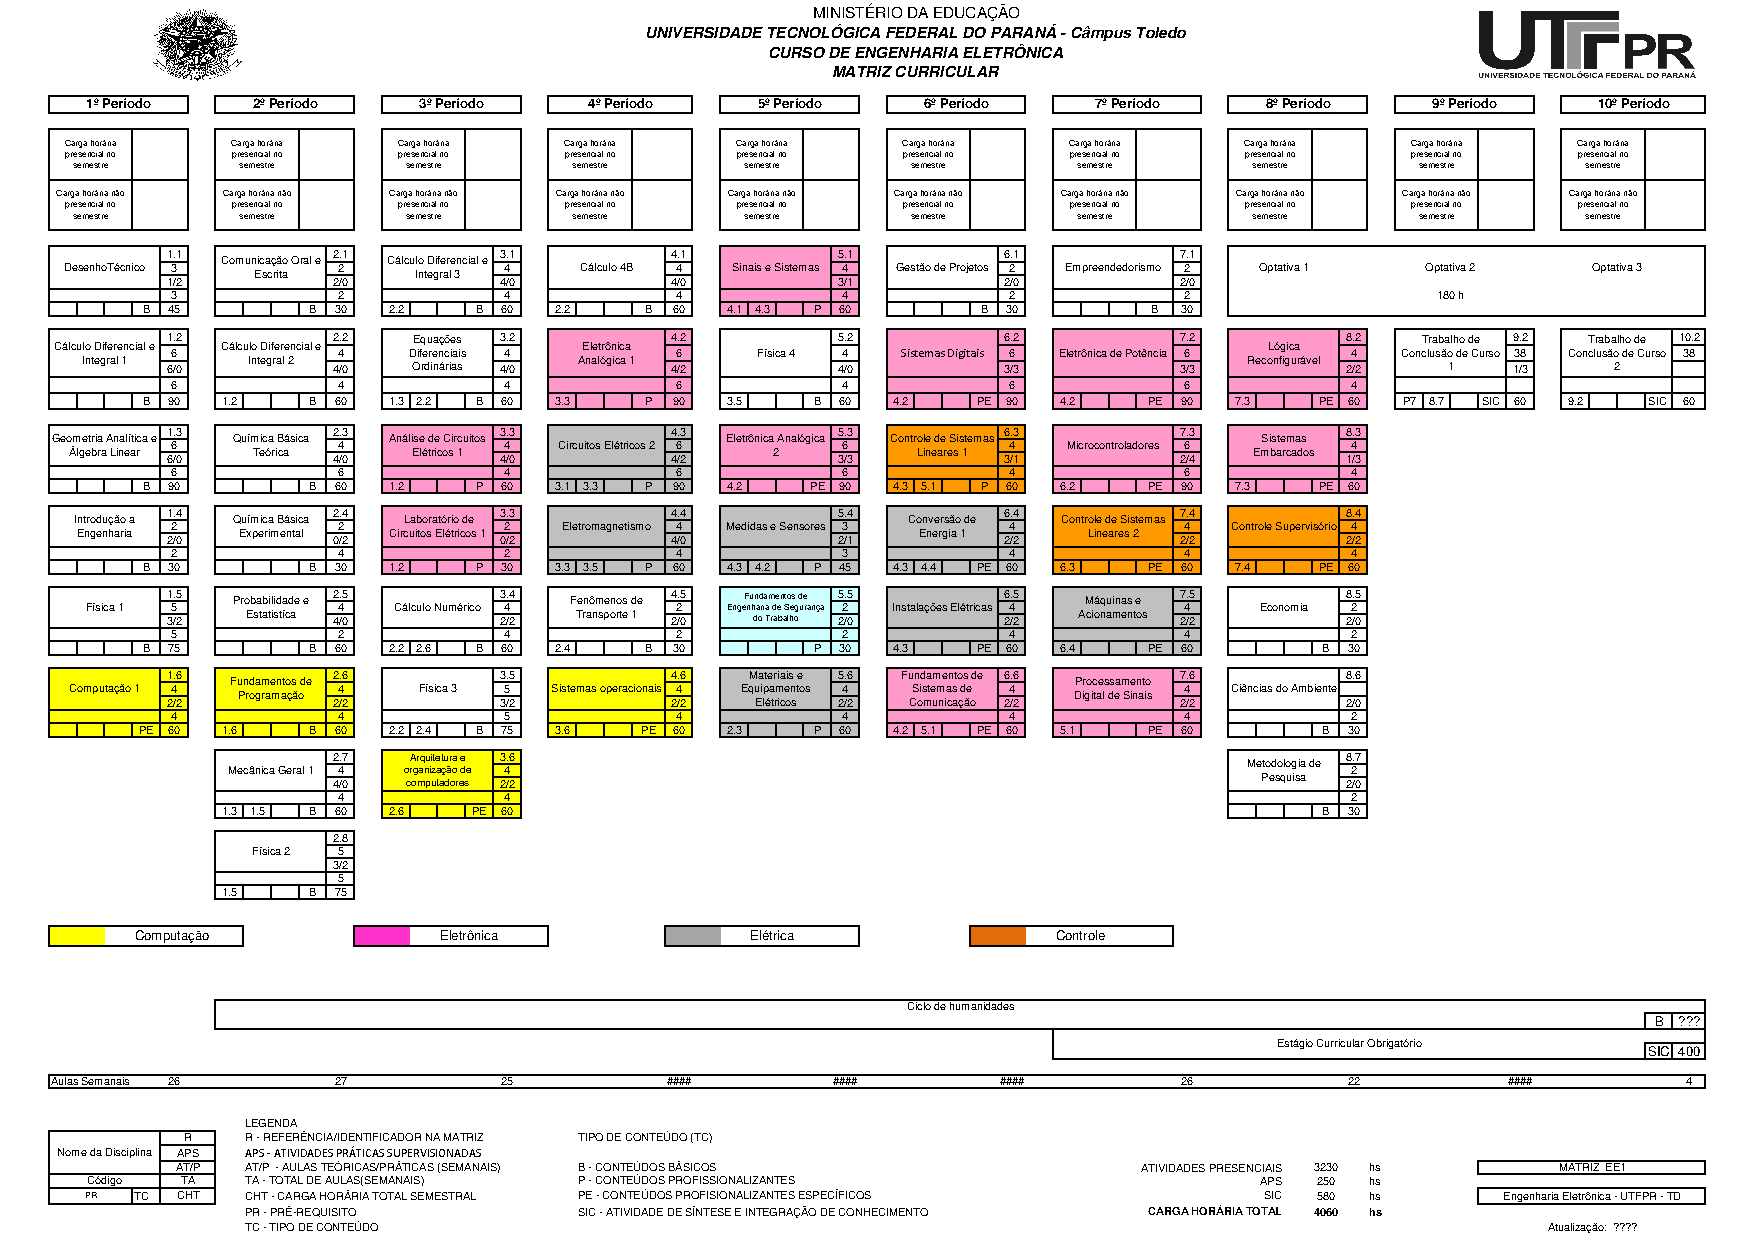
\includegraphics[width=1.2\textwidth]{Caps/Figs/NovaMatriz.pdf}
		\fonte{\utf}
		\label{qua:matriz}
	\end{quadro}
\end{landscape}

\subsection{Regime Letivo}
\label{sub:reg}

As atividades acadêmicas serão em regime semestral, com número mínimo de pré-requisitos, visando melhor consolidação dos conhecimentos nas áreas de atuação do engenheiro eletrônico. A matrícula no curso é realizada por disciplina. Quanto à matrícula e à periodização serão seguidas as normas institucionais do Regulamento de Organização Didático Pedagógica aplicável ao curso.

\subsection{Duração do curso}

Integralização mínima em 5 anos (10 períodos, sendo cada período equivalente a um semestre letivo) e máxima em 9 anos, de acordo com o Regulamento da Organização Didático Pedagógica dos Cursos de Graduação da UTFPR \cite{rodp}.

\subsection{Carga horária de atividades teóricas e práticas}

As atividades teóricas do curso compreendem \pdfmarkupcomment{2626 horas-aula}{Atualizar ao final, verificar a possibilidade de inserir uma tabela}. Destaca-se que, conforme a Instrução Normativa 02/10 da Instituição \cite{in2:2010:prograd}, uma aula na UTFPR possui 50 minutos. Assim sendo, foi realizada a compensação da duração de uma aula (50 minutos) em horas (60 minutos), dividindo o número total de horas-aula por 1,2.

\nomenclature[A]{PROGRAD}{Pró-reitoria de Graduação} 

As atividades práticas do curso compreendem \pdfmarkupcomment{1242 horas-aula}{atualizar ao final}. Todo ano é promovida a semana acadêmica com enfoque em atividades científicas, atividades de extensão, palestras e seminários com profissionais que atuam em áreas pertinentes à formação do discente e outros. Também são promovidas, de acordo com a disponibilidade, visitas técnicas durante o curso.

\subsection{Carga horária das Aulas à Distância (AD)}

Segundo portaria de MEC N\textordmasculine 2.117, de 6 de dezembro de 2019 \cite{portaria2117mec}, as instituições de ensino poderão ofertar disciplinas em no \pdfmarkupcomment{máximo 40\%}{inserir um quadro demonstrativo? A utfpr prevê ainda 20\%?} de sua carga horária total do curso. A principal ferramenta de Tecnologia de informação e comunicação (TIC) para a oferta desta modalidade é o sistema MOODLE. Para que uma disciplina ocorra desta maneira deve estar previsto em plano de ensino e ser aprovado por colegiado competente. Entretanto, em caso de ausência do docente por motivo previsto ou não previsto (como acidentes, doenças, falecimentos, dentre outros) a aula pode ser antecipada ou reposta por meio de uma atividade não presencial a distância desde que seja aprovada pelo coordenador do curso conforme Resolução n\textordmasculine 084/17 do COGEP \cite{cogep84}.

\nomenclature[A]{AD}{Aulas à distência}

\subsection{Carga horária do Estágio Curricular Obrigatório}

Segundo as Diretrizes Curriculares Nacionais dos Cursos de Graduação em Engenharia \cite{dcneng}, em seu artigo 11, ``a formação  do  engenheiro  inclui,  como  etapa  integrante da  graduação, as práticas reais, entre as quais o estágio curricular obrigatório sob supervisão direta do curso''. Aliado a essa diretriz, a UTFPR estabelece, na Resolução Conjunta COGEP-COEMP N\textordmasculine{} 01/2020, de 02 de junho de 2020 \cite{cogepcoemp1:2020}, que a carga horária mínima de estágio obrigatório para os cursos da UTFPR deve ser de 400 horas, sendo esse o mesmo valor adotado pelo curso de Engenharia Eletrônica.

\nomenclature[A]{COEMP}{Conselho de Ralações Empresariais e comunitárias}

\subsection{Carga horária do TCC}

O TCC tem uma carga total de 144 horas-aula, a carga horária é dividida igualmente nas disciplinas de TCC 1 e TCC 2.

\subsection{Carga horária de Atividade complementares}

\pdfmarkupcomment{Verificar se as Atividade complementares continuarão.}{segundo as DCNs, deve-se manter}

\subsection{Carga horária das Atividades de Extensão}
\label{sub:extch}

A curricularização da Extensão no curso, é desenvolvida como uma possibilidade de aplicação de um conjunto de conhecimentos desenvolvidos durante as atividades de ensino e pesquisa e ofertada para a comunidade universitária da UTFPR, à comunidade no entorno direto da Universidade e às regiões circunvizinhas.

As atividades de Extensão enfocam a observação da realidade, tratada com o objetivo de produzir impacto junto à comunidade visando o desenvolvimento regional sustentável. Estarão organizadas em torno de programas ou projetos, sendo incluídas no projeto individual de algumas disciplinas, \pdfmarkupcomment{totalizando 400 horas}{Atualizar ao final}.


\section{CONTEÚDOS CURRICULARES}

Esta seção descreve: os componentes curriculares por período; as unidades curriculares obrigatórias, optativas e eletivas, demonstrando a totalização das cargas horárias.  A composição da distribuição gradual dos períodos e áreas de conhecimento é apresentado em uma sequência didática lógica demonstrando a integração entre os componentes curriculares. Também é descrito como está estruturado o ciclo de humanidades (grupo de unidades curriculares da área de humanidades exigido pela Resolução 90 do COGEP \cite{cogep90}).


\subsection{Unidades Curriculares do Primeiro Período}

A \autoref{tab:per1} representa a distribuição das unidades curriculares do primeiro período do curso de Engenharia Eletrônica. %Os Quadros de \ref{qua:desenho} à \ref{qua:cicomp} apresentam os dados estruturais de cada unidade curriclar do referido período. 

% tabela de unidades curriculares do primeiro período
\begin{table}[htb!]
	\centering\tiny
	\caption{Conteúdos curriculares do Primeiro Período}
	\label{tab:per1}
	%
\begin{tabular}{cccccccc}
\toprule
% Cabeçalho
\multicolumn{3}{p{7cm}}{\thead{Primeiro Período}} & \multicolumn{5}{p{7cm}}{\thead{Carga horária (h)}}\\ \cmidrule(lr){1-3} \cmidrule(lr){4-8}
\multicolumn{1}{c}{\multirow{2}[3]{*}{\thead{Área de \\Conhecimento}}} & \multicolumn{1}{c}{\multirow{2}[3]{*}{\thead{Unidade Curricular}}} & \multicolumn{1}{c}{\multirow{2}[3]{*}{\thead{E*}}} & \multicolumn{2}{c}{\thead{Presencial}}& \multicolumn{2}{c}{\thead{Não\\ Presencial}} & \multicolumn{1}{c}{\multirow{2}[3]{*}{\thead{Total}}} \\ \cmidrule(lr){4-5} \cmidrule(lr){6-7}
& & & \thead{Teórica} & \thead{Prática} & \thead{Teórica} & \thead{Prática} & \\ \midrule

% dados
% área de conhecimento                  Disciplina                                              Extensão    Teórico Pre Prática Pre Teórico Dist    Prática dist    Total
\makecell{Ciclo de \\ humanidades}      & \makecell{Desenho Técnico}                            &           & 15        & 30        & -             & -             & 45 \\
\makecell{Matemática}                   & \makecell{Cálculo Diferencial \\ Integral 1}          &           & 90        & -         & -             & -             & 90 \\
\makecell{Matemática}                   & \makecell{Geometria Analítica \\ e Algebra Linear}    &           & 90        & -         & -             & -             & 90 \\
\makecell{Educação em \\ Engenharia}    & \makecell{Introdução à Engenharia \\ Eletrônica}      &\checkmark & 30        & -         & -             & -             & 30 \\
\makecell{Física}                       & \makecell{Física 1}                                   &           & 45        & 30        & -             & -             & 75 \\
\makecell{Ciência da \\ Computação}     & \makecell{Construção de \\ algorítimos}               &           & 30        & 30        & -             & -             & 60 \\



% Finalização
\midrule
\multicolumn{7}{r}{Carga Horária total do Período}   & 390 \\ 
\midrule
\multicolumn{7}{r}{Carga Horária total de Extensão}  & 30  \\
\bottomrule
\multicolumn{8}{l}{*Unidade Curricular extensionista}


\end{tabular}%

	\tabelaPeriodo{1}{Primeiro}
\end{table}

